\addchap{Regelmäßige Veranstaltungen auf dem Campus}
% TODO: Bin offen für andere Namen ^^

\minisec{Spieleabende}

Etwa einmal im Monat wird in der Fakultät vom FSR ein Spieleabend ausgerichtet. Start ist dabei immer um 18:30 Uhr im Foyer. Dabei stellt der FSR sein umfangreiches Angebot an analogen Spielen zur Verfügung, sodass eine ganze Menge an Spielen schon von Haus aus da sind. Wollt ihr etwas spielen, was nicht da ist, bringt es am besten mit! Oft sind auch schnell Leute gefunden, die mal ein neues Spiel ausprobieren wollen.

Hin und wieder finden sich auch ein paar Leute, die an dem Abend ihre Notebooks mitbringen und eine kleine LAN-Party schmeißen oder ihre Spielekonsole mitbringen, um über einen der Beamer der Seminarräume mit anderen zusammen zu spielen.

Für Knabbereien und Getränke wird gesorgt, das \emph{ascii} hat in der Regel zu Spieleabenden geöffnet. Wenn das Wetter mitspielt, ist auch das \emph{Count Down}, ein Dresdner Studentenclub, zur Stelle und verkauft Heißes vom Grill sowie alkoholische Getränke.

Es lohnt sich also auf jeden Fall, vorbei zu schauen und bei einer Mate und einer frischen Bratwurst neue Leute kennenzulernen!

\minisec{Stammtische}

\minisec{OUTPUT.DD}

\minisec{KIF}

\minisec{ESE}


\minisec{Studentenklub Count Down}

\begin{wrapfigure}{l}{3.25cm}%
  \vspace{-.5cm}
  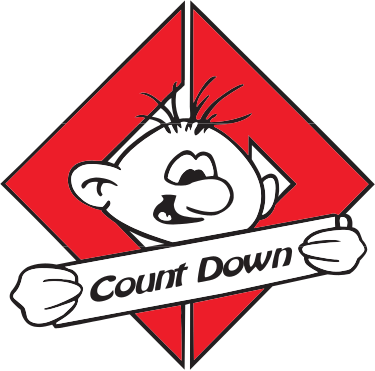
\includegraphics[width=\linewidth]{img/countdown}
  \vspace{-1cm}
\end{wrapfigure}

Um einen Ort für gemeinsame Treffen und Aktivitäten zu haben, betreibt der Studentenklub IZ e.V. das Count Down.
Dieses befindet sich im Keller des Wohnheims Güntzstraße 22 Eingang C und liegt damit auf halbem Weg zwischen Campus und Neustadt.
Mit einer Mischung aus gemütlichen Kneipenabenden und verschiedenen Partys begleitet es dein Studentenleben, selbstverständlich zu studentischen Preisen!

Montags findet ein traditioneller und fast schon nostalgischer Spieleabend statt.
Damit es nicht langweilig wird, hat das Count Down eine große Auswahl an verschiedenen Brett- und Kartenspielen parat.

Bei den Erasmus-Partys hast du jeden Dienstag die Gelegenheit, gemeinsam mit ausländischen Studenten zu feiern und deren Kulturen kennen zu lernen.

\begin{wrapfigure}{r}{6.9cm}%
  \vspace{-.4cm}
  \hspace{.03\linewidth}\includegraphics[width=.96\linewidth]{img/ese2013/cd.jpg}
  \vspace{-.4cm}
\end{wrapfigure}

Darüber hinaus gibt es auch viele Veranstaltungen, die nicht im festgeschriebenen Rhythmus stehen, aber trotzdem immer wieder stattfinden.
Dazu gehören unter anderem ein Skatturnier, Cocktail- und Werewolfabende in englischer Sprache, sowie der Metalalterabend.
Den aktuellen Plan findest du unter \link{https://countdown-dresden.de} und auf dem Flyer, den du in der ESE-Tüte gefunden hast ;-)

Du willst gern einmal selbst auf der Bühne stehen?
Ob mit der Blockflöte oder einem spannenden Reisebericht:
Auch dafür ist Platz im Klub und Kalender!

Und solltest du keine fremden Zuschauer haben wollen, sondern einfach mit deinen Freunden eine Party außerhalb deiner eigenen vier Wände geben, bist du ebenfalls beim Count Down genau richtig.
An allen Tagen, an denen keine Veranstaltung geplant ist (insbesondere am Freitag und Samstag), hast du die Möglichkeit, den Klub zu studentisch günstigen Preisen zu mieten, Barpersonal, Aufräumen und Putzen inklusive.
Schau einfach auf die Homepage und reservier' einen Termin!

Das reicht dir immer noch nicht?
Du möchtest das Studentenklubleben gern selbst mit gestalten?
Du triffst gerne viele neue, nette Leute?
Du hast vielleicht sogar weitere Ideen für interessante Veranstaltungen?
Du möchtest gern einmal selbst an der Bar stehen und dabei nicht den Chef im Nacken sitzen, sondern den Spaß im Vordergrund stehen haben?
Sprich die Mitglieder einfach direkt an, neue Mitglieder sind immer herzlich willkommen.

Ob als Gast oder als neues Mitglied - das Count Down freut sich, dich bald im Klub begrüßen zu dürfen.